% !TEX root=./report.tex

\subsection{Static calibration}

\ITS{} are inherently dependent on the calibration of the different sensors. 
To track and predict traffic the system has to know the poses of the different sensors relative to some reference coordinate system.
This enables the ITS to accurately measure the position of vehicles within the single sensor ranges and at the overlapping boundaries.

Previous experiments have shown that a calibration process based on an IMU is not feasible in our case. 
Instead we focus on a calibration procedure based on visual landmarks in the video feed.
The landmarks are mapped to their partially known world positions from high definition road maps. 

%%%%%%%%%%%%%%%%%%%%%%%%%%%%%%%%%%%%%%%%%%%%%%%%%%%%%%%%%%%%%%%%%%%%%%%%%%%%%%%%%%%%%%%%%%%%%%%%%%%%%%%%%%%%%%%%%%%%%%%%%%%%%%%%%%%%%%%%%%%%%%%%%%%%%%%%%%%%%%%%%

\paragraph{Retrive objects from the \HDmaps}
In this work we focus on the permanent delineator objects that are easily visible in the video feeds.

The world position of the objects can be retrieved using the mathematical operations defined in the \OD{} standard.

This gives us the the base origin point $o~=~(x, y, z)^T$ of the object in the transverse mercator projection \cite{proj}. 
The base origin point is the world position of the lower end of the object where it ends in the ground or another object.

Additionally we retrieve a directional heading axis $d~=~(x, y, z)^T$ and the height $h$ of the object.

These values enable us to approximate the real-world objects by sampling points $s \in S$ in world position along the center line of the object, where 
\begin{equation}
S = \{s | s = o + \lambda * d: \quad \lambda \in [0, h]\}
\end{equation}
%%%%%%%%%%%%%%%%%%%%%%%%%%%%%%%%%%%%%%%%%%%%%%%%%%%%%%%%%%%%%%%%%%%%%%%%%%%%%%%%%%%%%%%%%%%%%%%%%%%%%%%%%%%%%%%%%%%%%%%%%%%%%%%%%%%%%%%%%%%%%%%%%%%%%%%%%%%%%%%%%

\paragraph{Mapping objects to pixels}

To calibrate the camera we need to establish a mapping
\begin{equation}
  s_c \mapsto p_c \Leftrightarrow  {o_c, d_c, \lambda_c} \mapsto p_c
\end{equation}
from pixels $p_c~=~(u,v)^T \in P$ from the video stream to the corresponding sampled points $s_c$ from the object they belong to.

This leaves us with a set $C$ of correspondences $\{p_c,s_c\}$.

This mapping is currently done by human interaction and not fully automated. 
To minimize the work an aiding system to mark pixels was implemented that outputs a list of pixels that can easily be mapped to the list of objects.

\begin{figure}[t]
  \begin{center}
  % \fbox{\rule{0pt}{2in} \rule{0.9\linewidth}{0pt}}
     \includegraphics[width=\linewidth]{images/hd_map_mapping.png}
  \end{center}
     \caption{Left: The current camera frame. Right: A part of the \HDmaps{}. Cyan: The mapping $s_c \mapsto p_c$ from objects (right) to their corresponding pixels (left).}
  \label{fig:hd_map_mapping}
  \end{figure}

%%%%%%%%%%%%%%%%%%%%%%%%%%%%%%%%%%%%%%%%%%%%%%%%%%%%%%%%%%%%%%%%%%%%%%%%%%%%%%%%%%%%%%%%%%%%%%%%%%%%%%%%%%%%%%%%%%%%%%%%%%%%%%%%%%%%%%%%%%%%%%%%%%%%%%%%%%%%%%%%%

\paragraph{Relaxation of problem by line approximation}
\begin{figure*}[!ht]
  \centering
  \begin{tabular}{cc}
    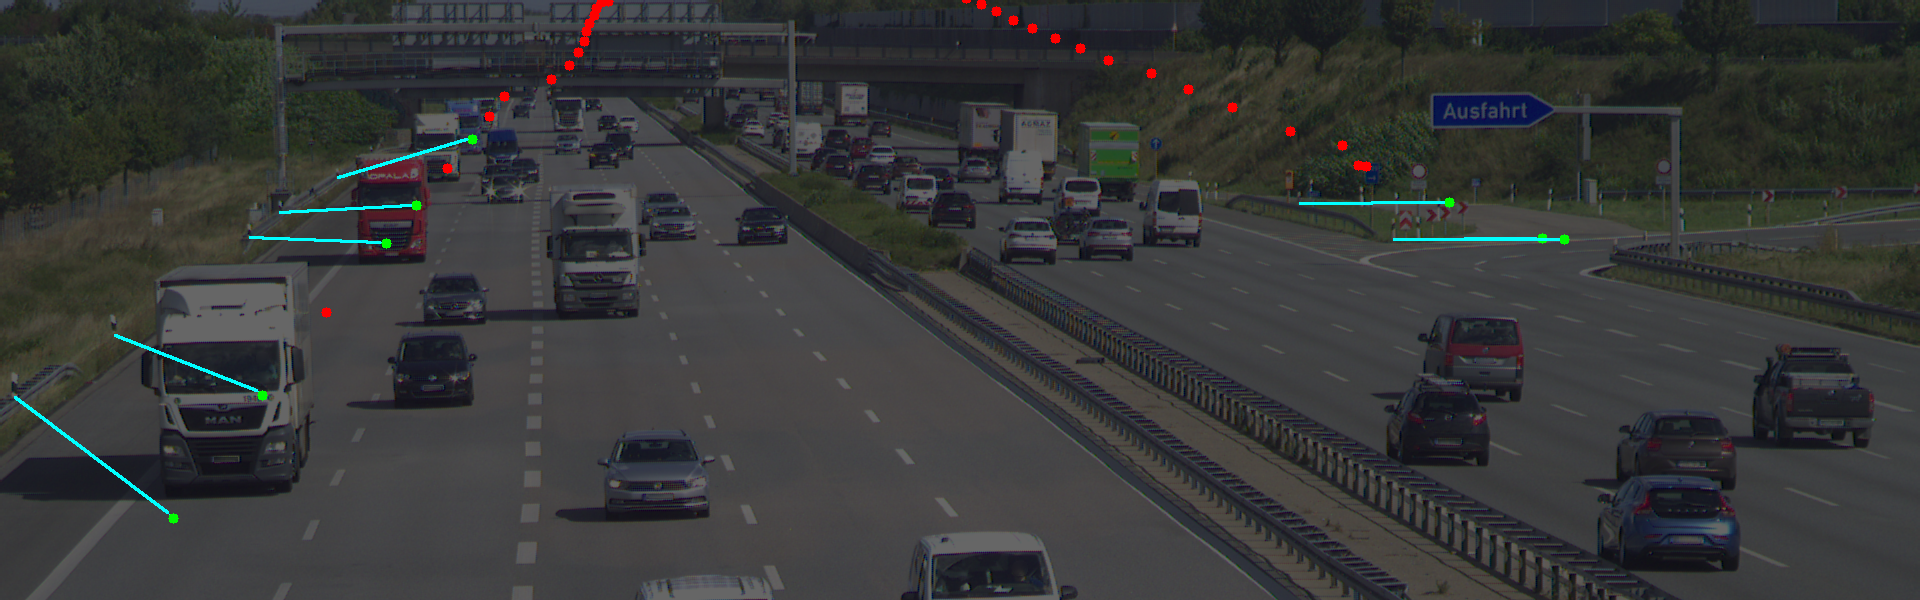
\includegraphics[width=0.475\linewidth]{images/calibration/background_uncalibrated_with_mapping.png}    &  
    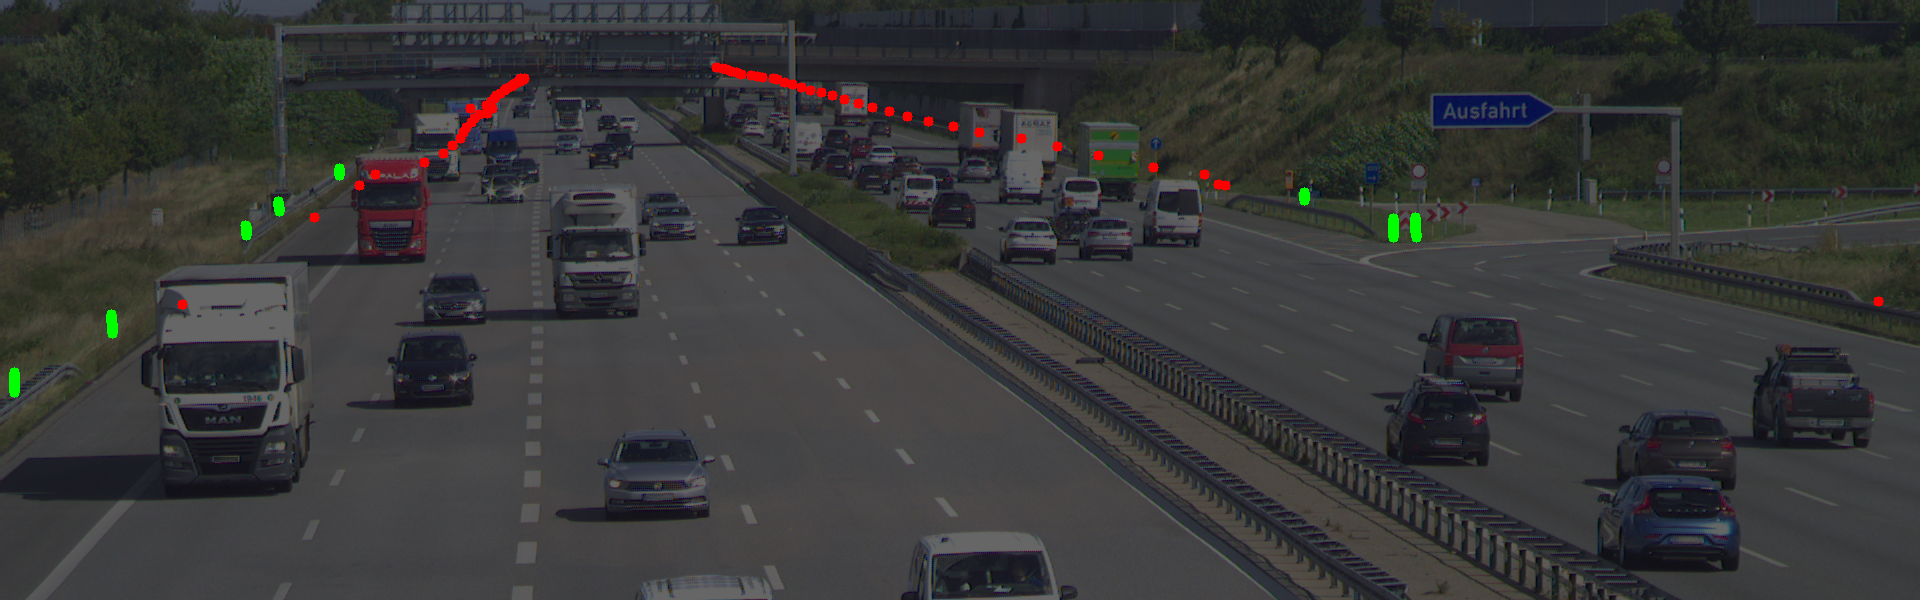
\includegraphics[width=0.475\linewidth]{images/calibration/background_calibrated.png}    
  \end{tabular}
  \caption{Left: Sampled points of objects that are mapped to pixel locations (green) and sampled points without known corresponding pixels (red) rendered by a poorly calibrated camera model.
  The mapping from the points to their expected pixels is drawn in cyan.
  Right: The same sampled points after the calibration procedure.
  The rendered positions of the sampled points align with the pixels of the objects they are mapped to and the drawn mapping disappears as the distance approaches $0$.  }
  \label{fig:calibration}
  \end{figure*}
Approximating the objects by lines removes the need for exactly known 3D correspondences as usually needed in calibration problems. 
Nonetheless it does not require to jointly estimate the full world position of the objects and camera pose jointly as in Bundle-Adjustment problems.
%
The assumptions we made are: 
\begin{itemize}
  \item Objects are symmetric around their directional heading axis.
  \item Pixels of the objects are also symmetric around the projected directional axis.
  \item The pixels in the mapping is equally distributed around the directional axis as the deviations from tangential offset points cancel out then. 
\end{itemize}

This models that the objects collapse into their center line in 2D and 3D and that tangentially deviating points on the surface in one direction equally cancels out by the opposite point mirrored at the center line.

%%%%%%%%%%%%%%%%%%%%%%%%%%%%%%%%%%%%%%%%%%%%%%%%%%%%%%%%%%%%%%%%%%%%%%%%%%%%%%%%%%%%%%%%%%%%%%%%%%%%%%%%%%%%%%%%%%%%%%%%%%%%%%%%%%%%%%%%%%%%%%%%%%%%%%%%%%%%%%%%%

\paragraph{Calibration procedure}
  
Our camera is modelled using the pinhole camera model. 
This uses the known intrinsic camera parameters and their corresponding projection $\pi$ from camera to image space.

The extrinsic camera parameters that map from world space to camera space are defined by the camera translation $T$ and the camera rotation $R$.
The translation and rotation are unknown, for them we optimize. 

We estimate the camera pose by minimizing a modified version of the reprojection error 
\begin{equation}
  \min_{T, R, \Lambda, W} E(P, S, T, R, \Lambda, W) 
\end{equation}
formulated as
\begin{equation}
  \begin{split}
    s_c =& o_c + \lambda_c * h_c \\
  E(P, S, T, R, \Lambda, W ) =& 
  \sum_{c \in C} 
  \left\lVert 
    w_c * [ p_c - \pi(T * R * s_c) ]
  \right\rVert_2^2 \\ 
  +& 
  \sum_{c \in C} 
  \left\lVert 
  penalize(\lambda_i, h_i)
  \right\rVert_2^2 \\ 
  +& 
  \sum_{c \in C} 
  \left\lVert 
  \alpha * (1 - w_i)
  \right\rVert_2^2 
\end{split}
\label{eq:reprojection_error}
\end{equation}
where $P$ is the set of mapped pixels in the image, $S$ is the set of mapped corresponding sampled points from the objects and $\Lambda$ is the set of $\lambda$ values associated with the sampled points.
This formulation allows the optimization over the line approximations of the objects and jointly optimizes for the camera parameters $T, R$ and the $\lambda \in \Lambda$ parameters of the line objects.

The calculation of the exact position of $s_c \sim \lambda$ allows the optimizer to search the whole space of real numbers for $\lambda$.
Nonetheless we penalize values for $\lambda$ that exceed the physical height of the object by 
\begin{equation}
    penalize(\lambda, h) =
    \begin{cases}
      \lambda - h,& \text{if } \lambda > h\\
      \lambda,    & \text{if } \lambda < 0\\
      0,    & \text{else}
    \end{cases} 
\end{equation}
This regularization enables a robust estimation procedure that can flexibly adjust to the missing exact world positions.

\paragraph{Initialization}
In contrast to most pose estimation problems our approach drops the need for good initialization. 
By regularization of the $\lambda$ values enough flexibility is given to optimize over an infinite space of values, 
but enforces the solution of the $\lambda$ to lie within the interval of $\lambda \in [0, h]$.

\begin{equation}
  \bar{s} = \frac{1}{\left\lvert C \right\rvert } \sum_{c \in C} o_c 
\end{equation}

\begin{equation}
  T_0 = \begin{pmatrix}
    1, 0, 0,& \bar{s}_x \\   
    0, 1, 0,& \bar{s}_y \\   
    0, 0, 1,& \bar{s}_z + 1000 \\   
    0, 0, 0,& 1   
  \end{pmatrix}
\end{equation}

\begin{equation}
  R_0 = \mathbb{I} ^ {4 \times 4}
\end{equation}

It is sufficient to initialize with $\lambda_c = 0$ for all correspondences.
The camera rotation is defined to be zero with the camera facing in negative world $z$ axis.
By placing the camera at some distance over the mean of the known object positions with zero rotation the optimization always converges to the desired minimum.

% \begin{itemize}
%   \item HD map based approach
%   \item Optimization algorithm, reprojection error between map and video 
%   \item Landmark extraction, mapping, pose estimation
%   \item Watersheder for pixel marking
%  translation can be  and initializing the camera at the some distance over the mean    
 % \end{itemize}